\chapter{Introducción específica}

Este capítulo presenta los protocolos de comunicación, componentes de hardware
y herramientas de software utilizados en el desarrollo del trabajo. Se detallan
las características y sus especificaciones técnicas.

%----------------------------------------------------------------------------------------
%	SECTION 1 - Protocolos de comunicación
%----------------------------------------------------------------------------------------

\section{Protocolos de comunicación}

En esta sección se describen los diferentes protocolos de comunicación
utilizados en el desarrollo del trabajo. 

\subsection{Wi-Fi}

Wi-Fi es el nombre comercial propiedad de la Wi-Fi Alliance para designar a su
familia de protocolos de comunicación inalámbrica basados en el estándar IEEE
802.11 para redes de área local sin cables \cite{Li2019}.

El estandar identifica dos modos principales de topología de red:
infraestructura y ad-hoc.

\begin{itemize}
	\item Modo infraestructura: los dispositivos se conectan a una red inalámbrica a
	      través de un router o AP (del inglés, \textit{Access Point}) inalámbrico, como
	      en las WLAN. Los AP se conectan a la infraestructura de la red mediante el
	      sistema de distribución conectado por cable o de manera inalámbrica.
	\item Modo ad-hoc: los dispositivos se conectan directamente entre sí sin necesidad
	      de un punto de acceso.
\end{itemize}

\subsection{MQTT}

MQTT es un protocolo de mensajería estándar internacional OASIS
\cite{OASIS_MQTT_Standard} para Internet de las Cosas (IoT). Está diseñado como
un transporte de mensajería de publicación/suscripción extremadamente ligero,
ideal para conectar dispositivos remotos con un consumo de código reducido y un
ancho de banda de red mínimo.

MQTT es un protocolo ligero basado en TCP/IP \cite{AWS_MQTT} que sigue un
modelo de publicación/suscripción, donde:

\begin{itemize}
	\item Broker: funciona como un servidor central que recibe los mensajes de los
	      clientes y los distribuye a los suscriptores correspondientes, actúa como
	      intermediario en la comunicación.
	\item Cliente: puede ser un dispositivo que publica mensajes en un tópico o que
	      recibe mensajes al estar suscrito a un tópico.
	\item Tópico: es la dirección a la que se envían los mensajes en MQTT. El broker se
	      encarga de distribuirlos a los clientes suscritos. Los temas se organizan en
	      una estructura jerárquica de tópicos.
\end{itemize}

\subsection{TLS}

TLS es un protocolo de seguridad criptográfica diseñado para garantizar la
privacidad y la integridad de los datos en comunicaciones sobre redes, como
Internet \cite{tls}. Opera sobre la capa de transporte y permite autenticación,
cifrado de datos y protección contra manipulación.

TLS se utiliza para garantizar la confidencialidad de los protocolos de
aplicación (MQTT \cite{OASIS_MQTT_Standard}, HTTP \cite{IBMTCPIP} y WebSocket
\cite{RFC6455}) \cite{awsiot_tls}.

%----------------------------------------------------------------------------------------
%	SECTION 2 - Componentes de hardware
%----------------------------------------------------------------------------------------

\section{Componentes de hardware}\label{sec:hardware}

En esta sección se describen los diferentes elementos de hardware utilizados en
el desarrollo del trabajo. 

\subsection{Microcontrolador}\label{sec:microcontrolador}

El microcontrolador ESP-WROOM-32 (figura \ref{fig:ESP32}), es un chip de tipo
SoC (del inglés, \textit{System on Chip}) de bajo costo y bajo consumo de
energía que integra Wi-Fi, Bluetooth y Bluetooth LE en un solo paquete. El
ESP-WROOM-32 \cite{EspressifESP32WROOM} es un microcontrolador de 32 bits con
una arquitectura Xtensa LX6 de doble núcleo, lo que le permite ejecutar dos
hilos de ejecución simultáneos. Además, cuenta con una amplia gama de
periféricos, como UART, I2C, SPI y ADC, que lo hace ideal para aplicaciones de
IoT.

\begin{figure}[H]
	\centering
	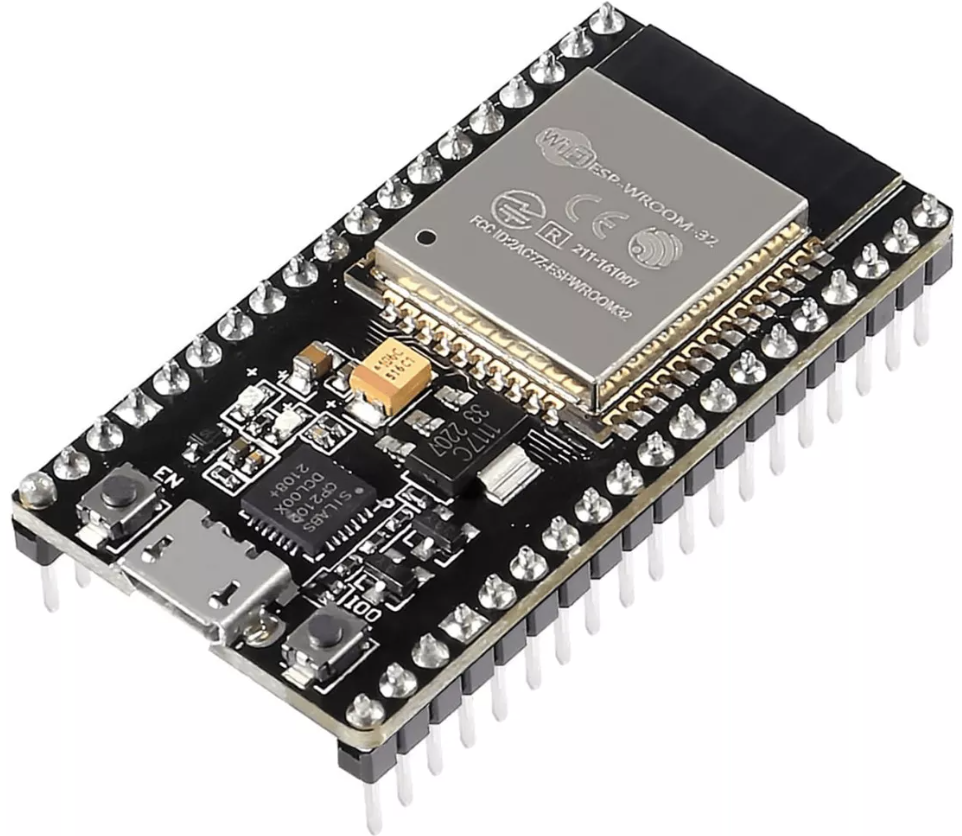
\includegraphics[height=.15\textwidth]{./Images/3.png}
	\caption{Microcontrolador ESP-WROOM-32\protect\footnotemark.}
	\label{fig:ESP32}
\end{figure}

\footnotetext{Imagen tomada de \href{https://www.hobbytronica.com.ar/MLA-916790826-nodemcu-esp32-wifi-bluetooth-42-iot-wroom-esp32s-arduino-_JM}
	{Nodemcu Esp32 Wifi HobbyTronica.}}

\subsection{Sensor de temperatura ambiente, humedad relativa y presión atmosférica}

El BME280 (figura \ref{fig:BME280}) es un sensor digital de alta precisión para
la medición de temperatura ambiente, humedad relativa y presión atmosférica. Se
comunica a través de las interfaces I2C y SPI y ofrece una precisión de ±1 °C
para la temperatura ambiente, ±3 \code{\%} para la humedad relativa y ±1 hPa
para la presión atmosférica \cite{BoschBME280}.

\begin{figure}[H]
	\centering
	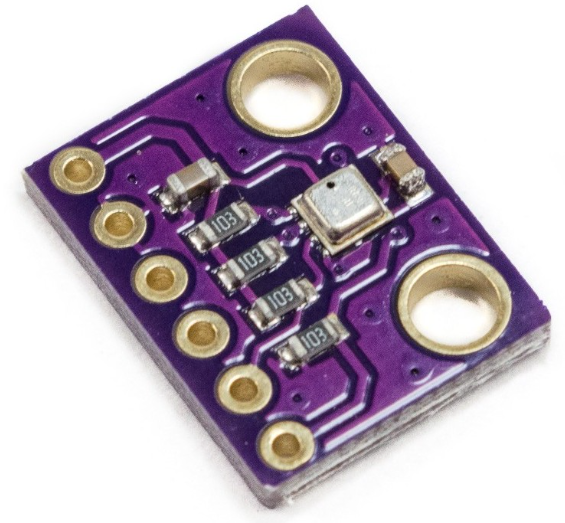
\includegraphics[height=.15\textwidth]{./Images/4.png}
	\caption{Sensor BME280\protect\footnotemark.}
	\label{fig:BME280}
\end{figure}

\footnotetext{Imagen tomada de \href{https://naylampmechatronics.com/sensores-posicion-inerciales-gps/357-sensor-bme280-presion-temperatura-y-humedad.html}
	{Sensor BME280 Naylamp Mechatronics.}}

\subsection{Sensor de luz digital}\label{sec:BH1750}

El BH1750 (figura \ref{fig:BH1750}) es un sensor digital de intensidad luminosa
que mide la iluminación ambiental en lux. Utiliza la interfaz I2C para la
comunicación y puede medir niveles de luz en un rango de 1 a 65.535 lux, con
una precisión de 1 lux \cite{ROHM_BH1750}.

\begin{figure}[H]
	\centering
	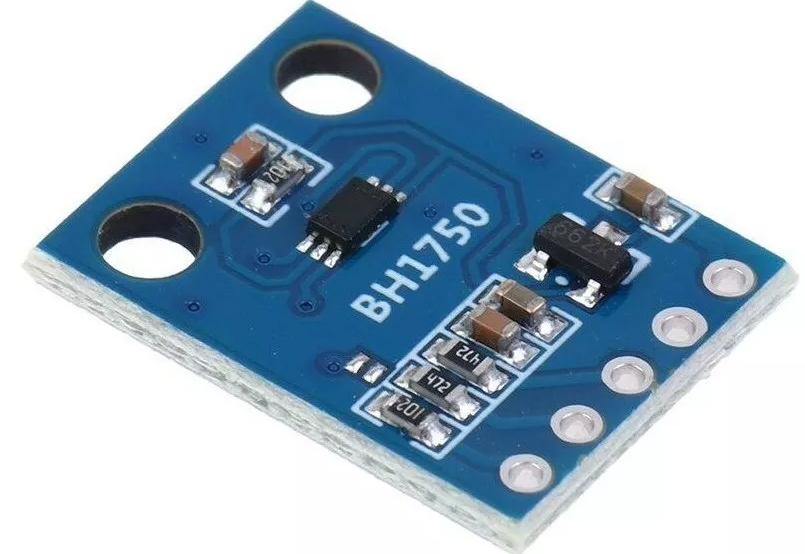
\includegraphics[height=.15\textwidth]{./Images/5.png}
	\caption{Sensor BH1750\protect\footnotemark.}
	\label{fig:BH1750}
\end{figure}

\footnotetext{Imagen tomada de \href{https://www.hobbytronica.com.ar/MLA-905448482-modulo-sensor-de-luz-digital-ambiente-bh1750-gy-302-arduino-_JM}
	{Sensor BH1750 HobbyTronica.}}

\subsection{Sensor de dióxido de carbono}

El sensor MH-Z19C (figura \ref{fig:MHZ19C}) es un detector de $CO_2$ por NDIR
(del inglés, \textit{Non Dispersive Infrared Detector}). Se comunica a través
de la interfaz UART y es capaz de medir la concentración de $CO_2$ en un rango
de 0 a 5000 ppm con una precisión de 50 ppm \cite{WINSEN_MHZ19C}.

\begin{figure}[H]
	\centering
	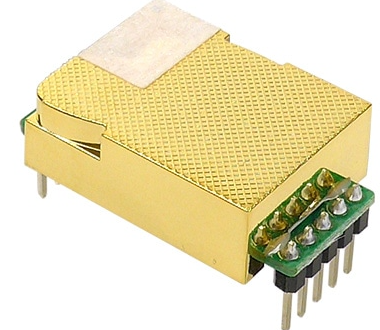
\includegraphics[height=.15\textwidth]{./Images/6.png}
	\caption{Sensor MHZ19C\protect\footnotemark.}
	\label{fig:MHZ19C}
\end{figure}

\footnotetext{Imagen tomada de \href{https://qiita-image-store.s3.ap-northeast-1.amazonaws.com/0/130771/54be6203-1014-ba5e-3a6f-86e3a403c472.png}
	{MH-Z19C PartsCabi.net.}}

\subsection{Sensor de detección de pH}

El sensor PH-4502C (figura \ref{fig:PH4502C}) mide la acidez o alcalinidad del
líquido mediante un electrodo de vidrio. Se comunica a través de la interfaz
analógica y es capaz de medir el pH en un rango de 0 a 14 \cite{PH-4502C}.

\begin{figure}[H]
	\centering
	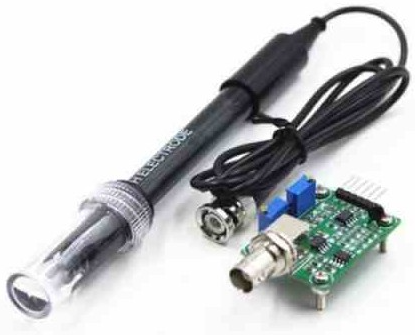
\includegraphics[height=.15\textwidth]{./Images/7.png}
	\caption{Sensor PH-4502C\protect\footnotemark.}
	\label{fig:PH4502C}
\end{figure}

\footnotetext{Imagen tomada de \href{https://http2.mlstatic.com/D_NQ_NP_755250-MLM42784110936_072020-O.webp}
	{Sensor PH-4502C Mercado Libre Static.}}

\subsection{Sensor de conductividad eléctrica}

El sensor de CE (figura \ref{fig:CE}) mide la capacidad de una solución para
conducir electricidad, lo que depende de la presencia de iones. A mayor
concentración de iones, mayor es la conductividad \cite{MTConductivitySensor}.
Este sensor se comunica a través de una interfaz analógica y puede medir la
conductividad en un rango de 0 a 20 mS/cm \cite{EC-Sensor}.

\begin{figure}[H]
	\centering
	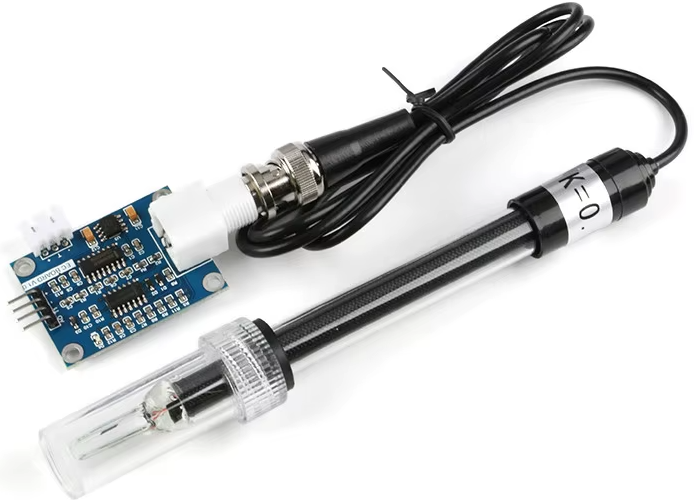
\includegraphics[height=.15\textwidth]{./Images/8.png}
	\caption{Sensor CE\protect\footnotemark.}
	\label{fig:CE}
\end{figure}

\footnotetext{Imagen tomada de \href{https://m.media-amazon.com/images/I/51dAS-cD01L._AC_SL1000_.jpg}
	{Sensor CE Amazon.}}

\subsection{Sensor de sólidos disueltos totales}

El sensor TDS (figura \ref{fig:TDS}) mide la cantidad de sales, minerales y
metales que se encuentran disueltos en la solución \cite{TDS-description}. Se
comunica a través de la interfaz analógica y es capaz de medir la concentración
de TDS en un rango de 0 a 1000 ppm \cite{TDS-Sensor}.

\begin{figure}[H]
	\centering
	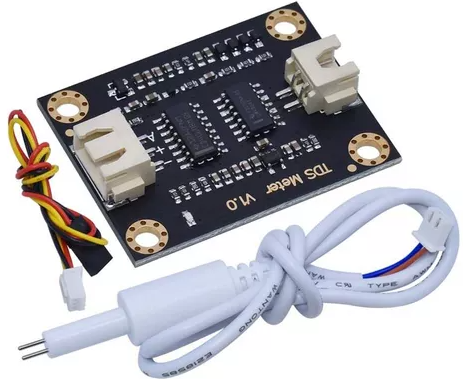
\includegraphics[height=.15\textwidth]{./Images/9.png}
	\caption{Sensor TDS\protect\footnotemark.}
	\label{fig:TDS}
\end{figure}

\footnotetext{Imagen tomada de \href{https://es.aliexpress.com/i/1005003343459012.html?gatewayAdapt=glo2esp}
	{Sensor TDS Aliexpress.}}

\subsection{Sensor de temperatura digital sumergible}

El DS18B20 (figura \ref{fig:DS18B20}) es un sensor digital de temperatura
sumergible. Se comunica a través de la interfaz \textit{OneWire} y puede medir
la temperatura en un rango de -55 °C a 125 °C con una precisión de ±0.5 °C
\cite{DS18B20}.

\begin{figure}[H]
	\centering
	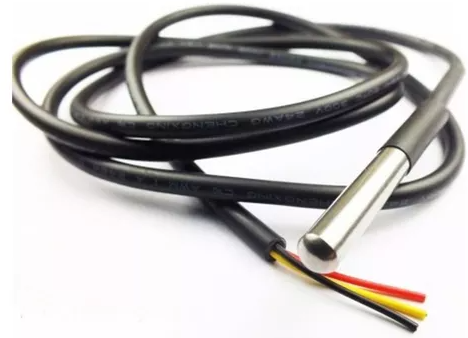
\includegraphics[height=.15\textwidth]{./Images/10.png}
	\caption{Sensor de temperatura DS18B20\protect\footnotemark.}
	\label{fig:DS18B20}
\end{figure}

\footnotetext{Imagen tomada de \href{https://articulo.mercadolibre.com.ar/MLA-1904241050-sensor-de-temperatura-ds18b20-sumergible-con-cable-de-2-m-_JM}
	{Sensor DS18B20 Mercado Libre.}}

\subsection{Sensor ultrasónico}

El sensor HC-SR04 (figura \ref{fig:HC-SR04}) mide distancias por ultrasonido en
un rango de 2 cm a 400 cm con una precisión de 3 mm. Se comunica a través de la
interfaz GPIO \cite{HC-SR04}.

\begin{figure}[H]
	\centering
	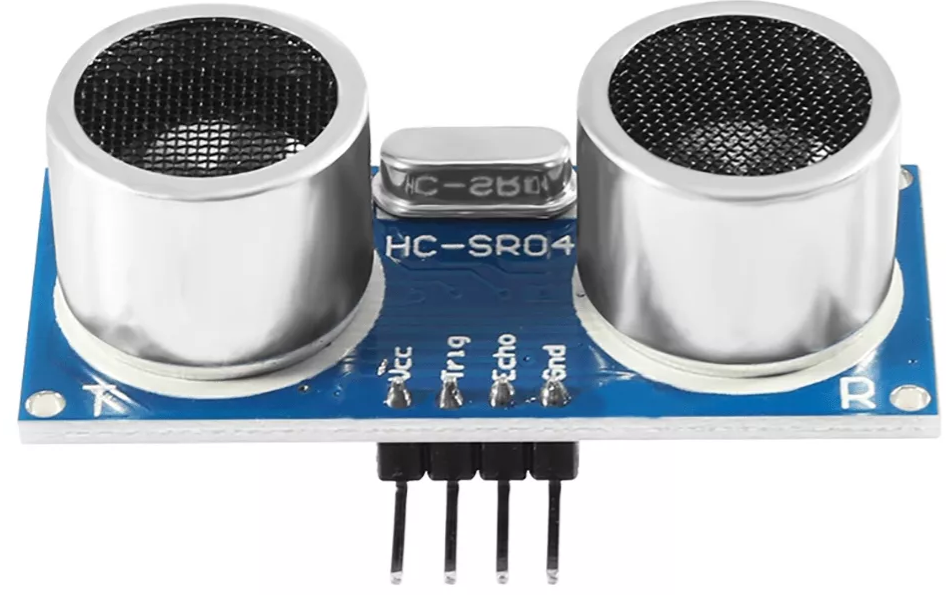
\includegraphics[height=.15\textwidth]{./Images/11.png}
	\caption{Sensor HC-SR04\protect\footnotemark.}
	\label{fig:HC-SR04}
\end{figure}

\footnotetext{Imagen tomada de \href{https://es.aliexpress.com/item/1005007542287447.html}
	{Sensor HC-SR04 Aliexpress.}}

\subsection{Sensor de medición de consumo eléctrico}

El sensor PZEM-004T (figura \ref{fig:PZEM-004T}) es un módulo de medición de
parámetros eléctricos que mide la tensión, corriente, potencia activa y energía
consumida. Se comunica a través de la interfaz UART y es capaz de medir la
tensión en un rango de 80 a 260 V, la corriente en un rango de 0 a 100 A, y la
potencia en un rango de 0 a 22 kW \cite{PZEM-004T}.

\begin{figure}[H]
	\centering
	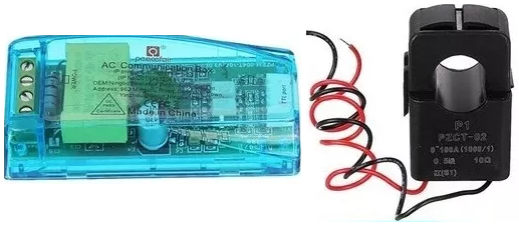
\includegraphics[height=.15\textwidth]{./Images/12.png}
	\caption{Sensor de medición de consumo eléctrico\protect\footnotemark.}
	\label{fig:PZEM-004T}
\end{figure}

\footnotetext{Imagen adaptada de \href{https://articulo.mercadolibre.com.ar/MLA-908885966-modulo-monitoreo-energia-monofasico-pzem-004t-elegir-_JM}
	{Sensor PZEM-004T Mercado Libre.}}

\subsection{Módulo de relés}

El módulo de relés (figura \ref{fig:Relé}) es un actuador eléctrico de dos
canales optocoplados que permite el control de encendido y apagado de
dispositivos eléctricos. Se comunica a través de la interfaz GPIO y es capaz de
controlar dispositivos de hasta 10 A y 250 VAC \cite{Relé}.

\begin{figure}[H]
	\centering
	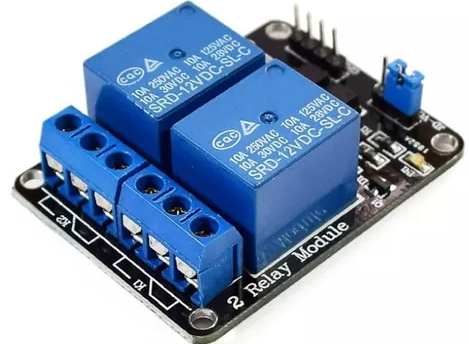
\includegraphics[height=.15\textwidth]{./Images/13.png}
	\caption{Relé de 2 Canales 5 V 10 A\protect\footnotemark.}
	\label{fig:Relé}
\end{figure}

\footnotetext{Imagen tomada de \href{https://www.amazon.com.mx/MV-ELECTRONICA-RELEVADOR-Canales-LOWLEVEL/dp/B07PR7XHWT}
	{Relé de 2 Canales Amazon.}}

%----------------------------------------------------------------------------------------
%	SECTION 3 - Componentes de software
%----------------------------------------------------------------------------------------

\section{Desarrollo de firmware}

En esta sección se describe la herramienta de software utilizada para la
programación de los microcontroladores ESP32.

\subsection{MicroPython}

MicroPython es una implementación optimizada de Python 3 para
microcontroladores y sistemas embebidos. Está diseñado para ejecutarse en
dispositivos con recursos limitados, como el ESP32, y proporciona una forma
sencilla de programar microcontroladores con un lenguaje de alto nivel como
Python \cite{MicroPython}.

Su facilidad de uso, la amplia disponibilidad de bibliotecas y la reducción del
tiempo de desarrollo lo convierten en una opción eficiente. Además, al ser un
lenguaje interpretado, posibilita la ejecución interactiva de pruebas y
depuración, facilitando la identificación y corrección de errores en el código
\cite{CTAMicroPython}.

%----------------------------------------------------------------------------------------
%	SECTION 4 - Desarrollo Backend y API
%----------------------------------------------------------------------------------------

\section{Desarrollo backend y API}

En esta sección se presentan las herramientas de software utilizadas en el
desarrollo del backend y la API REST.

\subsection{FastAPI}

FastAPI es un framework moderno para la construcción de APIs REST rápidas y
escalables en Python. Está diseñado para ser fácil de usar, rápido de
desarrollar y altamente eficiente en términos de rendimiento. FastAPI utiliza
Python 3.6+ y aprovecha las características de tipado estático de Python para
proporcionar una API autodocumentada y con validación de tipos integrada
\cite{FastAPI}.

\subsection{MongoDB}

MongoDB es una base de datos NoSQL (del inglés, \textit{Not Only SQL}) de
código abierto y orientada a documentos que proporciona una forma flexible y
escalable de almacenar y recuperar datos. Utiliza un modelo de datos basado en
documentos que almacena datos en un formato similar a JSON (del inglés,
\textit{JavaScript Object Notation}) llamado BSON (del inglés, \textit{Binary
	JSON}) que permite almacenar datos de forma anidada y sin esquema fijo, lo que
facilita la manipulación y consulta de datos no estructurados \cite{MongoDB}.

%----------------------------------------------------------------------------------------
%	SECTION 5 - Desarrollo Frontend
%----------------------------------------------------------------------------------------

\section{Desarrollo frontend}

En esta sección se presentan las herramientas de software utilizadas en el
desarrollo del frontend.

\subsection{React}

React es una biblioteca de JavaScript de código abierto para construir
interfaces de usuario interactivas y reutilizables. Desarrollada por Facebook,
React permite crear componentes de interfaz de usuario que se actualizan de
forma eficiente cuando cambian los datos, lo que facilita la creación de
aplicaciones web rápidas y dinámicas \cite{React}.

%----------------------------------------------------------------------------------------
%	SECTION 6 - Infraestructura y despliegue
%----------------------------------------------------------------------------------------

\section{Infraestructura y despliegue}

En esta sección se presentan las herramientas de software utilizadas en la
infraestructura y despliegue del sistema.
\subsection{Docker}

Docker es una plataforma de código abierto que permite a los desarrolladores y
a los equipos de operaciones construir, empaquetar y desplegar aplicaciones en
contenedores. Los contenedores son unidades de software ligeros y portátiles
que incluyen todo lo necesario para ejecutar una aplicación, incluidas las
bibliotecas, las dependencias y el código \cite{Docker}.

Docker facilita la creación de entornos de desarrollo y despliegue consistentes
y reproducibles, lo que garantiza que las aplicaciones se ejecuten de la misma
manera en cualquier entorno.

\subsection{AWS IoT Core}

AWS IoT Core es un servicio de AWS (del inglés, \textit{Amazon Web Services})
que permite a los dispositivos conectarse de forma segura a la nube y
comunicarse entre sí a través de protocolos de comunicación estándar como MQTT
y HTTP. Proporciona una infraestructura escalable y segura para la gestión de
dispositivos, la recopilación de datos y la integración con otros servicios de
AWS \cite{AWS_IoT}. Utiliza TLS para cifrar la comunicación entre los
dispositivos y la nube, para garantizar la confidencialidad y la integridad de
los datos.

\subsection{AWS EC2}

Amazon EC2 (del inglés, \textit{Elastic Compute Cloud}) es un servicio de AWS
que proporciona capacidad informática escalable en la nube. Permite a los
usuarios lanzar instancias virtuales en la nube con diferentes configuraciones
de CPU, memoria, almacenamiento y red, lo que facilita la implementación de
aplicaciones escalables y de alta disponibilidad \cite{AWS_EC2}.

%----------------------------------------------------------------------------------------
%	SECTION 7 - Herramientas de desarrollo
%----------------------------------------------------------------------------------------

\section{Herramientas de desarrollo}

En esta sección se presentan las herramientas de software utilizadas en el
desarrollo del sistema.

\subsection{Visual Studio Code}

Visual Studio Code, comúnmente abreviado como VS Code, es un entorno de
desarrollo integrado (IDE, del inglés, \textit{Integrated Development
	Environment}) de código abierto, altamente extensible y multiplataforma
compatible con Windows, macOS y Linux \cite{VSCode}.

VS Code es un editor de código ligero y rápido con soporte para muchos
lenguajes de programación y extensiones que permiten personalizar y mejorar la
funcionalidad del editor. Además, cuenta con herramientas de depuración
integradas, control de versiones y terminal integrada.% cientos de

\subsection{Postman}

Postman es una plataforma de colaboración para el desarrollo de APIs que
permite a los desarrolladores diseñar, probar y documentar de forma rápida.
Proporciona una interfaz gráfica intuitiva para enviar solicitudes HTTP a un
servidor y visualizar las respuestas, lo que facilita la depuración y el
desarrollo de APIs \cite{Postman}.

\subsection{GitHub}

GitHub es una plataforma de alojamiento de repositorios Git \cite{Git} que
permite a los desarrolladores colaborar en proyectos de software de forma
distribuida. Proporciona herramientas para gestionar el código fuente, realizar
seguimiento de los cambios, revisar el código, realizar integración continua y
despliegue automático \cite{Github}.

